% Author: David Larsen <dcl9934@cs.rit.edu>
\documentclass[11pt]{article}
\usepackage{fullpage}
\usepackage{listings}
\usepackage{needspace}
\usepackage{color}
\usepackage{ifthen}
\usepackage{graphicx}


\lstset{ %
basicstyle=\footnotesize,       % the size of the fonts that are used for the code
numbers=left,                   % where to put the line-numbers
stepnumber=1,                   % the step between two line-numbers. If it's 1 each line will be numbered
numbersep=5pt,                  % how far the line-numbers are from the code
showspaces=false,               % show spaces adding particular underscores
showstringspaces=false,         % underline spaces within strings
tabsize=4,		                % sets default tabsize to 4 spaces
language=Python
}

\ifthenelse{\isundefined{\isAnswerKey}}
{
    \newenvironment{answer}{\large\lstset{basicstyle=\large}\color{white}}{}
}
{
    \newenvironment{answer}{\large\lstset{basicstyle=\large}\color{red}}{}
}


\author{Computer Science Community}

\begin{document}
\noindent{\Large CS-241 Midterm Exam Review \hfill \today}

\begin{enumerate}
    \item\label{reverse()} Write a function which reverses a string (e.g. ``Don't
        get sick'' becomes ``kcis teg t'noD'').

\begin{answer}
\begin{lstlisting}
def reverse( string ):
    if string == '' :
        return string
    else:
        return reverse( string[1:] ) + string[0]
\end{lstlisting}
\end{answer}

    \item Perform a substitution trace on 
    \begin{lstlisting}
    reverse('Cinco-fone')
    \end{lstlisting}
%\needspace{15\baselineskip}

\begin{answer}
\begin{lstlisting}
reverse('Cinco-fone')
reverse('inco-fone') + 'C'
reverse('nco-fone') + 'i' + 'C'
reverse('co-fone') + 'n'  + 'i' + 'C'
reverse('o-fone') + 'c' + 'n'  + 'i' + 'C'
reverse('-fone') + 'o'  + 'c' + 'n'  + 'i' + 'C'
reverse('fone') + '-'  + 'o'  + 'c' + 'n'  + 'i' + 'C'
reverse('one') + 'f' + '-'  + 'o'  + 'c' + 'n'  + 'i' + 'C'
reverse('ne') + 'o' + 'f' + '-'  + 'o'  + 'c' + 'n'  + 'i' + 'C'
reverse('e') + 'n' + 'o' + 'f' + '-'  + 'o'  + 'c' + 'n'  + 'i' + 'C'
'e' + 'n' + 'o' + 'f' + '-'  + 'o'  + 'c' + 'n'  + 'i' + 'C'
'enof-ocniC'
\end{lstlisting}
\end{answer}
\pagebreak
    \item Define a function that takes an input string and rotates the sequence
        of letters in each word by n. For example: shift\_left(``DEADBEEF'', 3)
        will produce the output string ``DBEEFDEA''. \\ shift\_left("Giant Robot", 4) will produce "t RobotGian"\\ 
        shift\_left("X", 5) will produce "X" \\You should be able to
        shift a string by a value greater than the length of the
        string\footnote{The \% operator, which finds the remainder of a
        division operation will be useful here.}.\\ 
        \emph{Assume a function len( str ) which returns the length of a string is provided}


    \begin{enumerate}
        \item Design: Give brief description on how your function should
            accomplish this.

            \begin{answer}
            Our implementation will grab the first part of the new string by
            slicing all characters at an index after the offset. The second
            part of the string will be all of the characters up to the offset
            point. We will then concatenate the two strings.

            Making it possible for the offset to be greater than the length of
            the string can be accomplished by making {\tt offset = offset mod
            len(string)}
            \end{answer}

        \item Testing: Provide 3 test cases, using specific values for the input
            string and amount of shifting and what the expected output should be
            for each.

            \begin{answer}
                shift\_left(``'', 5) should return ""\\
                shift\_left(``A'',5) should return "A"\\
                shift\_left(``ABADCAFE'',300) == shift\_left("ABADCAFE",4)\\
                shift\_left(``FOO'', 1) should return "OOF"
            \end{answer}

        \item Implement the function in Python.

\begin{answer}
\begin{lstlisting}
def shift_left(string, offset):
    if len(string) == 0:
        return string
    else:
        offset = offset % len(string)
        first = string[offset:]
        last = string[:offset]
        return first + last
\end{lstlisting}
\end{answer}

        \item Implement the function {\tt shift\_right()}, which rotates letters
            in the opposite direction.

\begin{answer}
\begin{lstlisting}
def shift_right(string, offset):
    return shift_left(string, -offset)
\end{lstlisting}
\vspace{0.5in}
\end{answer}

    \end{enumerate}
\pagebreak
    \item Write a function that takes in a file name, and returns the average
        size of a word in that file. The files will only have 1 word per line,
        for example:

        \begin{center}
        No\\
        soup\\
        for\\
        you!
        \end{center}

        which has an average length of: 3.25 \\ \emph{Assume a function len( str ) which returns the length of a string is provided}


\begin{answer}
\begin{lstlisting}
def average_wordlength(filename):
    characters = 0
    words = 0
    for line in open(filename):
        words += 1
        characters += len(line)
    return characters/words
\end{lstlisting}
\end{answer}

    \item Write a function that takes in a string representation of a number and returns the sum
        of all of digits in the string. \\For example sum( '11111' ) returns 5. \\
        \emph{Assume a function len( str ) which returns the length of a string is provided. \\
         assume a function int( str ) which, given a string representation of an integer, returns its integer value }

        \begin{enumerate}
            \item Recursively.
\begin{answer}
\begin{lstlisting}
def sumRec( numbers ):
    if len( numbers ) == 0:
        return 0
    else:
        return int(numbers[0]) + sumRec( numbers[1:] )
\end{lstlisting}
\end{answer}

            \item Iteratively
\begin{answer}
\begin{lstlisting}
def sumIt( numbers ):
    total = 0
    while numbers != '':
        total += int( numbers[0] )
        numbers = numbers[1:]
    return total
\end{lstlisting}
\end{answer}
            \item How would you test this function?
                \begin{answer}
                \begin{itemize}
                    \item Empty string 
                    \item String length = 1
                    \item string length $>$ 1
                \end{itemize}
                \end{answer}
\pagebreak
\end{enumerate}
\item Assuming the turtle is facing east, write the python code to draw the following picture given the proper depth as input:
    \begin{itemize}
            \item depth = 0
           \\No output 
            \item depth = 1\\
            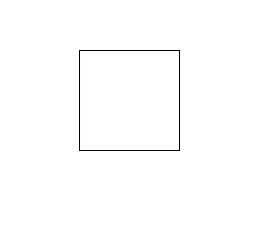
\includegraphics[scale=0.4]{1.png}
            \item depth = 2 \\
            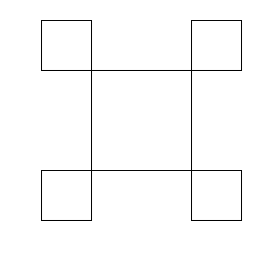
\includegraphics[scale=0.4]{2.png}
            \item depth = 3\\
            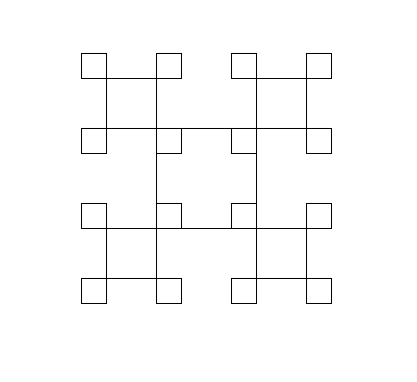
\includegraphics[scale=0.4]{3.png}
        \end{itemize}
    \begin{answer}
    \begin{lstlisting}
       def drawSqaures( length, depth ):
           if depth <= 0:
               return
           count = 4
           while count > 0:
               turtle.forward( length )
               turtle.left( 90 )
               drawSqaures( length/2, depth-1 )
               turtle.right( 180 )
               count -= 1
      \end{lstlisting}
     \end{answer}

    \item What does the following evaluate to?
    \begin{lstlisting}
def writeThatDown( n ):
    if n < 5:
        return n
    return (2 * n)

def he( n ):
    temp = n + 180
    if temp > 185:
        return temp
    return n

def putstheFernback( n ):
    return -n

n = 20
n = he(putstheFernback(writeThatDown( n ) ) )
print( n )
    \end{lstlisting}
    \begin{answer}
        -40
    \end{answer}

\item Write a function which performs a basic string compression, which uses counts of repeated characters. For example 
the string $abbbccccaaa$ would be compressed to: $a1b3c4a3$. 
 \emph{Assume a function len( str ) which returns the length of a string is provided. \\
      assume a function int( str ) which, given a string representation of an integer, returns its integer value. \\
      Assume a function str( int ) which, given an integer, returns the string representation of this integer, is provided. }

\begin{answer}
\begin{lstlisting}
def compress( string ):
    new = ''
    curChar = string[0]
    count = 0
    for char in string:
        if char == curChar:
            count += 1
        else:
            new = new + curChar + str(count)
            curChar = char
            count = 1 

    new = new + curChar + str(count)
    return new
\end{lstlisting}
\end{answer}
\newpage
\item Below is python code for a function that performs an insertion sort
    and prints ``data'' after each iteration of the for-loop.
\begin{lstlisting}
def insertion_sort( data ):
    for marker in range( 1, len( data ) ):
        val = data[marker]
        i = marker
        while i > 0 and data[i-1] > val:
            data[i] = data[i-1]
            i -= 1
        data[i] = val
        print( data )
\end{lstlisting}
        Write out what the function will print for the input list: [3,2,7,1].
\pagebreak
\item What is the time complexity on the previous sorting algorithm?

 \end{enumerate}
\end{document}
